\documentclass[english]{beamer}

\usepackage[utf8]{inputenc} 
\usepackage[T1]{fontenc}
\usepackage{lmodern}
\usepackage{amsmath,amssymb,amsthm}
\usepackage{dsfont}
\usepackage{babel}
\usetheme{Singapore}
\usepackage{bbm,multimedia,tikz}
\setbeamersize{text margin left=7pt,text margin right=7pt}
\usecolortheme{orchid}
\usepackage{amsmath,amssymb,amsthm}
\usepackage{setspace}
\usepackage{array}
\usepackage{hyperref}
%\usepackage{subfigure}
\usepackage{subcaption}
\usepackage{graphicx}
\usepackage{algorithm2e}
\usepackage{xcolor}
\setbeamercolor{block body}{use=structure,fg=black,bg=white}
\usepackage{cancel}
\usepackage{bigints}

\title[]{Some remarks on Generative Models}

%\author[]{***}
\date{\today}



\newcommand{\R}{\mathbb{R}}
\newcommand{\ind}{\mathbb{I}}
\newcommand{\EE}{\mathbb{E}}
\newcommand{\KL}{\mathrm{KL}}
\newcommand{\RC}{\mathrm{RC}}
\newcommand{\C}{\mathrm{C}}

\newcommand{\JS}{\mathrm{JS}}
\newcommand{\Div}{\text{Div}}


\newcommand{\Kinf}{\mathcal{K}_{\inf}}
\newcommand{\kl}{\mathrm{kl}}
\newcommand{\PP}{\mathbb{P}}
\newcommand{\Q}{\mathbb{Q}}

\renewcommand{\geq}{\geqslant}
\renewcommand{\leq}{\leqslant}
\newcommand{\m}{\mathrm{m}}
\newcommand{\mset}{\mathcal{M}\bigl([0,M]\bigr)}
\newcommand{\msetfin}{\mathcal{M}_{\mathrm{fin}}\bigl([0,M]\bigr)}
\newcommand{\eps}{\varepsilon}
\renewcommand{\d}{\mathrm{d}}
\newcommand{\algo}{\texttt}
\newcommand{\cA}{\mathcal{A}}
\newcommand{\cK}{\mathcal{K}}
\newcommand{\cX}{\mathcal{X}}
\newcommand{\cF}{\mathcal{F}}
\newcommand{\cZ}{\mathcal{Z}}
\newcommand{\cU}{\mathcal{U}}
\newcommand{\tX}{\widetilde{X}}
\newcommand{\cN}{\mathcal{N}}
\newcommand{\cQ}{\mathcal{Q}}
\newcommand{\Ng}{\mathcal{N}}

\newcommand{\uDelta}{\underline{\Delta}}
\renewcommand{\o}{\mathrm{o}}
\renewcommand{\O}{\mathrm{O}}
\newcommand{\nuzero}{\underline{\underline{\nu}}}
\newcommand{\cW}{\mathcal{W}}
\newcommand{\tw}{\widetilde{w}}
\newcommand{\pset}{\mathcal{P}[0,1]}

\newcommand{\hnu}{\widehat{\nu}}
\newcommand{\hmu}{\widehat{\mu}}
\newcommand{\mustar}{\mu^\star}
\newcommand{\astar}{a^*}

\DeclareMathOperator*{\argmax}{arg\,max}
\DeclareMathOperator*{\argmin}{arg\,min}

\renewcommand{\epsilon}{\varepsilon}
\newcommand{\ort}{\perp\!\!\!\perp}
\newcommand{\expg}[1] {\,{}^{#1}\! }
\newcommand{\logln}{\log\log}
%\newcommand{\kinnf}[args]{def}
\newcommand{\dpdq}{\frac{dP}{dQ}}
\newcommand{\tx}{\widetilde{x}}
\newcommand{\tz}{\widetilde{z}}
\newcommand{\tZ}{\widetilde{Z}}

\newcommand{\var}{\mathrm{Var}}
\newcommand{\papertitle}{Rapport de stage }
\newcommand{\esp}{\mathbb{E}}
\renewcommand{\phi}{\varphi}
\renewcommand{\abstractname}{gzegzeh}
\newcommand{\dnudnuprm}{\frac{d\nu_i}{d\nu_i'}}
%\renewcommand{\insertnavigation}[1]{}
\newtheorem{proposition}{Proposition}
\newcommand{\unu}{\underline{\nu}}


\makeatletter
\newcommand\mysphere{%
  \parbox[t]{10pt}{\raisebox{0.2pt}{\beamer@usesphere{item projected}{bigsphere}}}}
\makeatother

\newcommand{\comment}[1]{%
  \text{\phantom{(#1)}} \tag{#1}
}

\begin{document}
\RestyleAlgo{ruled}

\begin{frame}
	\titlepage

\end{frame}

%\begin{frame}
%    \frametitle{Plan}
%    \tableofcontents[hideallsubsection]
%\end{frame}

\section{The problem}
\subsection*{ }
\begin{frame}{Motivation}

Data $X_1,X_2,\ldots,X_K\textrm{ i.i.d }\sim P_X$. \textcolor{blue}{Learn to sample from $P_X$ ?}
\uncover<2->{

\vspace{0.5em}
$\to$ Easy, sample $I\sim\cU[1,K]$ generate $\tX = X_I$
}
\uncover<3->{

\vspace{1em}
Generalize to sample that are not in the dataset ? 
}
\uncover<4->{

\vspace{0.5em}
$\to$ Easy, fit parametric family of distribution with density $(q_{\theta})_{\theta\in\Theta}$
\[\hat{\theta}\in\argmax_{\theta\in\Theta}\sum_{k=1}^K\log\big(q_\theta(X_k)\big)\,,\]

then sample $\tX\sim q_{\hat{\theta}}$ $\to$ not so easy.
}
\end{frame}



\begin{frame}{Generative model}
    Data $X\sim P_X$ on $\cX$\qquad Feature $Z\sim P_Z$ on $\cZ$ \qquad Noise $N\sim P_N$ on $\cN$
\uncover<2->{    
    \textbf{Generator:} 
    \begin{align*}
        G: \cZ \times\cN &\to \cX\\
        (Z,N) &\mapsto G(Z,N)
    \end{align*}

}
\uncover<3->{
\begin{center}
\textcolor{blue}{Generated data $G(Z,N) =: \tX \sim P_{\tX}$}
\end{center}

\textbf{Goal:} Find $G$ such that 
\[  \textcolor{red}{P_X = P_{\tX}}\]

\textbf{Question/remarks:}

We don't know $P_X$ neither $P_{\tX}$, only \textcolor{red}{samples}.

Which loss for this problem? How to optimize it?

Do we want plausible samples? Nice features? 
}
\end{frame}


\section{GAN}
\subsection*{ }
\begin{frame}{GAN}
Data $X\sim P_X$ on $\cX$\qquad Feature $Z\sim P_Z$ on $\cZ$ \qquad Noise $N\sim P_N$ on $\cN$

\vspace{0.5em}
\textbf{Generator} $\textcolor{blue}{G(Z,N)=\tX\sim P_{\tX}}$

\qquad\textit{Goal:} Find G s.t. \qquad\qquad$P_{\tX}=P_X$
\vspace{0.02\textwidth}
\uncover<2->{

\textbf{Discriminator:} $\textcolor{blue}{D: \cX \mapsto [0,1]}$, \quad\quad\quad$Y\sim\mathcal{B}(1/2)$

\quad\quad\textit{Goal:} Find D s.t.
\[\textcolor{red}{D\bigr(Y X+(1-Y) G(Z,N)\bigr)\approx\PP\bigr(Y=1|Y X + (1-Y) G(Z,N)\bigl)}\]
}
\uncover<3->{
Log \only<3>{loss}\only<4->{\textcolor{blue}{gain}} for $D$:
\[
\only<3>{-\EE\biggl[Y\log\bigl(D(X)\bigr)+(1-Y)\log\Bigl(1-D\bigl(G(Z,N)\bigr)\Bigl)\biggr]}\only<4>{\textcolor{red}{V(D,G)=\EE\biggl[Y\log\bigl(D(X)\bigr)+(1-Y)\log\Bigl(1-D\bigl(G(Z,N)\bigr)\Bigl)\biggr]}}
\,.
\]
}
\uncover<4->{
Minimax objective
\[
\textcolor{red}{\min_{G}\max_{D} V(D,G)}\,.
\]}   
\end{frame}


\begin{frame}{Divergences}

Kullback-Leibler divergence between $P$ and $Q$
\[
\KL(P,Q) = \left\{\begin{array}{ll}
	\displaystyle \bigintsss_{\Omega} \ln\!\left(\frac{\d P}{\d Q}\right)\! \d P & \textrm{if $P \ll Q$}, \smallskip \\
	+ \infty & \textrm{else}.
\end{array} \right.
\]

Jensen-Shannon divergence between $P$ and $Q$
\[
\JS(P,Q) = \frac{1}{2}\KL\left(P,\frac{P+Q}{2}\right)+\frac{1}{2}\KL\left(Q,\frac{P+Q}{2}\right)
\]
\end{frame}

\begin{frame}

\begin{align*}
    V(D,G)&=\EE\biggl[Y\log\bigl(D(X)\bigr)+(1-Y)\log\Bigl(1-D\bigl(G(Z,N)\bigr)\Bigl)\biggr]\\
    &= \int_{\cX} \frac{1}{2}\log(D)\d P_X+\frac{1}{2}\log\big(1-D\big)\d P_{\tX}\, \d x
\end{align*}
\uncover<2->{

Optimal discriminator: 
\[
\only<2-3>{\textcolor{blue}{D_G^{*}=\argmax_{D} V(D,G)=\frac{\d P_X}{\d P_X+\d P_{\tX}}}}
\only<4>{
\textcolor{red}{D_{G^*}^{*}=\argmax_{D} V(D,G^*)=\frac{1}{2}}
}
\]
\hspace{0.01\textwidth}Objective at $G^*$:
\[
\textcolor{blue}{V(D_G^*,G)=\JS(P_X,P_{\tX})-\log(2)}
\]
}
\uncover<3->{

Global minimum 
\begin{align*}
    \textcolor{red}{G^*=\argmin_G V(D_G^*,G)\quad }&\textcolor{red}{\Leftrightarrow\quad  P_X = P_{\tX}}
    \end{align*}}
\end{frame}


\section{f-GAN}
\subsection*{ }


\begin{frame}{From variational formula to GAN}
\textbf{Kullback-Leibler:} Donsker-Varadhan formula and weak version \textcolor{blue}{$\phi^\star = \log (\d P /\d Q)$}
\begin{align*}
    \KL(P,Q) &= \sup_\phi \EE_P[\phi] -\log\EE_Q[e^\phi]\\
    &=\textcolor{blue}{\sup_\phi \EE_P[\phi+1] -\EE_Q[e^\phi]}
\end{align*}
\uncover<2->{
\textbf{reverse Kullback-Leibler:} only a weak version \textcolor{blue}{$\phi^\star = 1-\d Q/\d P$}
\begin{align*}
\KL(Q,P) = \textcolor{blue}{\sup_{\phi < 1} \EE_P [ \phi - 1] + \EE_Q[ \log(1-\phi) +1]}
\end{align*}}
\uncover<3->{
\textbf{Jensen-Shannon:} \textcolor{blue}{$\phi^\star = \log\big(\d P /(\d P +\d Q)\big)$}
\begin{align*}
    2 \JS(P,Q) -\log(4) &= \textcolor{blue}{\sup_{\phi \leq 0 } \EE_P[\phi] + \EE_Q\log(1-e^\phi)}\\
&= \sup_{0<D<1}\EE_P\log(D) + \EE_Q\log(1-D)
\end{align*}}
\end{frame}


\begin{frame}{Generalization to any $f$-divergence}
$f$-divergence between $P$ and $Q$ with $f$ convex, $f(1)=0$
\[
\Div_f(P,Q) = \displaystyle \bigintsss_{\Omega} f\!\left(\frac{\d P}{\d Q}\right)\! \d Q 
\]
\uncover<2->{
Variational formula: 
\[
\textcolor{blue}{
\Div_f(P,Q)=\sup_{\phi \in \Phi} \EE_P[\phi]- \EE_Q[f^*(\phi)]}\,,
 \]
where $\Phi$ is a well chosen class of functions and $f^*$ is the Fenchel conjugate of $f$ defined by 
\[
f^*(t) = \sup_{u\in \text{dom}_f} u t -f(u)\,.
\]
}

\end{frame}


\section{$\KL$ vs reverse-$\KL$}
\subsection*{ }
\begin{frame}{Learn to sample}
Assume we know $P_X$ and its density $p_X$.
\vspace{1em}

\textbf{Goal:} Generate plausible sample $\tx$ i.e. \textcolor{blue}{maximize the loglikelihood of this sample $\log\!\big(p_X(\tx)\big)$}
\vspace{0.5em}

If $\tx\sim p_{\tX}$, we want to minimize the  \textcolor{blue}{expected  negative loglikelihood}\uncover<2->{  + \textcolor{red}{ regularization}}
\begin{equation*}
    \textcolor{blue}{\int \log\left( \frac{1}{p_X}\right) p_{\tX}}\uncover<2->{ + \textcolor{red}{\int \log(p_{\tX}) p_{\tX}} = \KL(P_{\tX}),P_X}
\end{equation*}
\uncover<2->{
$\to$ reverse Kullback-Leibler divergence!}
\end{frame}

\begin{frame}{$\KL$ vs reverse-$\KL$}
It is the same to minimize $\min_Q \KL(P,Q)$ or $\min_Q \KL(Q,P)$ ?
\only<1> {
Yes !
\[
P = \argmin_{Q} \KL(P,Q) = \argmin_{Q} \KL(Q,P)
\]
}
\uncover<2->{

\vspace{1em}
But if we approximate $P$ with $Q\in \cQ$, for example
\[
P = \alpha \Ng(\mu_1,1)+(1-\alpha)\Ng(\mu_2,1) \qquad \cQ= \{\Ng(\mu,\sigma^2):\ \mu,\sigma\in\R\times\R^+\}
\]

\begin{figure}
    \centering
    \begin{subfigure}[t]{0.5\textwidth}
        \centering
        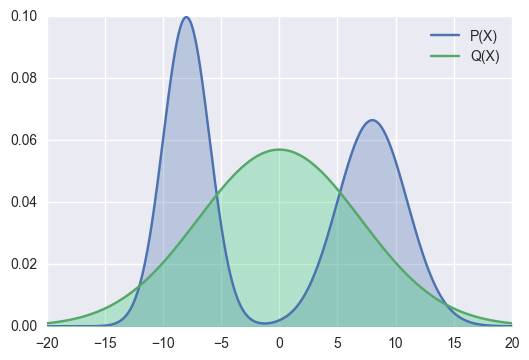
\includegraphics[height=1.5in]{fig/forward_1.png}
        \caption{Forward $P \ll Q$}
    \end{subfigure}%
    ~ 
    \begin{subfigure}[t]{0.5\textwidth}
        \centering
        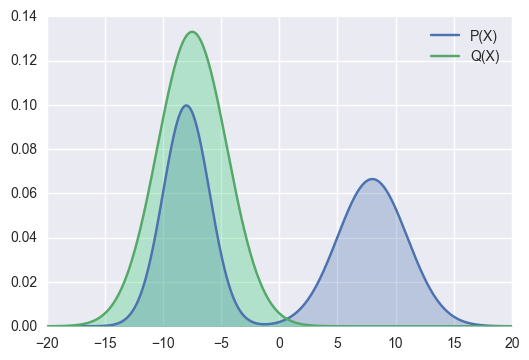
\includegraphics[height=1.5in]{fig/reverse.png}
        \caption{Reverse $Q \ll P$}
    \end{subfigure}
\end{figure} 
}
\end{frame}

\begin{frame}
\textbf{Sampling:}  $\min_{Q}\KL(Q,P)$

\vspace{1em}
But we don't know $P$ !  only samples $X_1,X_2,\ldots ,X_K \sim P_X$ $\to$ estimation
\vspace{1em}
\uncover<2->{
\textbf{Estimation:} $\min_{Q} \KL(P,Q)$

\vspace{1em}
Both ? $\to$ Jensen-Shannon divergence ?
\begin{align*}
\JS(P_X,P_{\tX}) &= \frac{1}{2} \KL\left(P_X,\frac{P_X+P_{\tX}}{2}\right) + \frac{1}{2}\KL\left(P_{\tX},\frac{P_X+P_{\tX}}{2}\right)\\
&= \inf_{Q } \frac{1}{2} \KL(P_X,Q) + \frac{1}{2}\KL(P_{\tX},Q)\,.
\end{align*}
\textcolor{red}{Nothing more than a vague intuition!}
}
\end{frame}

\begin{frame}{More on JS divergence}
Weighted Jensen-Shannon divergence:
\[
\JS^w(P,Q) = w \KL\big(P, w P + (1-w) Q\big) + (1-w) \KL\big(Q, w P+(1-w) Q\big) 
\]
Reverse Chernoff Information
\begin{align*}
    \textcolor{red}{\RC(P,Q)} &= \sup_{w\in[0,1]}\JS^w(P,Q)\\
    &= \inf_{Q'} \max\big(\KL(P,Q'),\KL(Q,Q')\big)\\
    &= \textcolor{red}{\KL(P,Q_\star)=\KL(Q,Q_\star)}
\end{align*}
Chernoff information
\[
\textcolor{blue}{\C(P,Q)= \KL(Q^\star,P)=\KL(Q^\star,Q)}
\]
\end{frame}


\section{VAE}
\subsection*{ }
\begin{frame}{Model}
\textbf{Feature to data:} \textcolor{blue}{$Z \sim P_Z \to G(Z,N)=\tX \sim P_{\tX|Z}$}

$(\tX,Z)\sim p_{(\tX,Z)}$ of density: $\textcolor{red}{p(x|z)}q(z)$  (formal...)  
\uncover<2->{

\vspace{1em}
\textbf{Data to feature:} \textcolor{blue}{$X \sim P_X \to \tZ \sim P_{\tZ|X}$}

$(X,\tZ)\sim p_{(X,\tZ)}$ of density: $p(x)\textcolor{red}{q(z|x)}$   
}
\uncover<3->{

\vspace{1em}
Usually $q$ is fixed, we need to parametrize $\big(p_\theta(x|z)\big)_{\theta\in\Theta}$ and $\big(q_\lambda(z|x)\big)_{\lambda\in\Lambda}$  

\vspace{1em}
\textit{In practice: }
\[q = \Ng(0,I) \]
\[
\quad \textcolor{red}{p_\theta(\cdot,z) = \Ng\Big(\mu_\theta(z), \text{diag}(\sigma^2_\theta(z)) \Big)} \quad q_\lambda(\cdot,x) =  \Ng\Big(\mu_\lambda(x), \text{diag}(\sigma^2_\lambda(x)) \Big)
\]
}
\end{frame}


\begin{frame}{Variationnal auto-encoder}

\textbf{Goal:} We want $P_{X, \tZ} = P_{\tX, Z}$ $\to$ \textbf{Loss: } $\textcolor{red}{\KL(P_{X,\tZ},P_{\tX,Z})}$ 

\vspace{1em}
\textbf{Tractable rewriting}

\begin{align*}
    \KL(P_{X,\tZ},P_{\tX,Z}) &= \int \log\!\left(\frac{p(x)q_\lambda(z|x)}{p_\theta(x|z)q(z)}\right)p(x)q_\lambda(z|x)\d x\d z\\
    &= \textcolor{red}{\int \KL\big(q_\lambda(z,x),q(z)\big)p(x)\d x}\\
    &\textcolor{red}{- \int\log\Big(p_\theta(x|z)\Big)q_\lambda(z|x)p(x)\d z\d x} +\textcolor{orange}{\int\log\big(p(x)\big)p(x) \d x}
\end{align*}
%    = \int \left( \int \log\left(\frac{q_\lambda(z|x)}{q(z)}\right)q_\lambda(z|x)- \log\Big(p_\theta(x|z)\Big)q_\lambda(z|x) +\log\!\big(p(x)\big)   \right)\d x
Therefore 
\begin{align*}
    \text{VAE loss}(\theta,\lambda) = \EE_{x\sim p(\cdot)}\left[ \KL\big(q_\lambda(z,x),q(z)\big) - \EE_{z\sim p_\theta(\cdot|x)}\big[\log\!\big(p_\theta(x|z)\big)\big] \right]
\end{align*}
\end{frame}
\end{document}